% 2010 年天津卷理科第 15 题：三角形 ABC 与点 D（D 在 BC 上，AD⊥AB）。
% 来源 PDF：普通高考/2010/2010天津理.pdf，SHA-256 340aba76699a12f330637f9c682abbc893e03e0e91788287934c0a7e0a3cace9。
% 原页：第 1 页（A3 六栏）第 3 栏中部，书页码 635。
% 重绘依据：B、D、C 共线，A 在 BC 上方，AD⊥AB；D 为 BC 内一点。
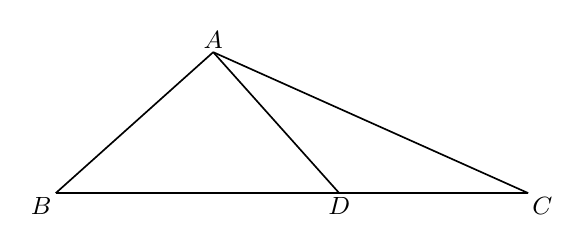
\begin{tikzpicture}[semithick, every node/.style={inner sep=1.2pt, font=\small}]
  \coordinate (B) at (0,0);
  \coordinate (C) at (6,0);
  \coordinate (D) at (3.6,0);
  \coordinate (A) at (2,1.79);
  \draw (B) -- (C);
  \draw (A) -- (B);
  \draw (A) -- (C);
  \draw (A) -- (D);
  \node[above] at (A) {$A$};
  \node[below left] at (B) {$B$};
  \node[below right] at (C) {$C$};
  \node[below] at (D) {$D$};
\end{tikzpicture}
